\subsection{Iterator (\textit{o Cursor})}
\label{iterator}

\textbf{Scopo}: Comportamentale \\
\textbf{Raggio d'azione}: Oggetti

\paragraph{Definizione} Il pattern Iterator fornisce un'interfaccia di accesso sequenziale agli elementi di un oggetto composito (es. collezioni) senza esporne la struttura interna. È bene notare che una classe che accede all’oggetto composito attraverso tale interfaccia non dipende dalla classe che implementa l’interfaccia e da quella che definisce l’oggetto composito.

\begin{figure}[H]
    \centering
    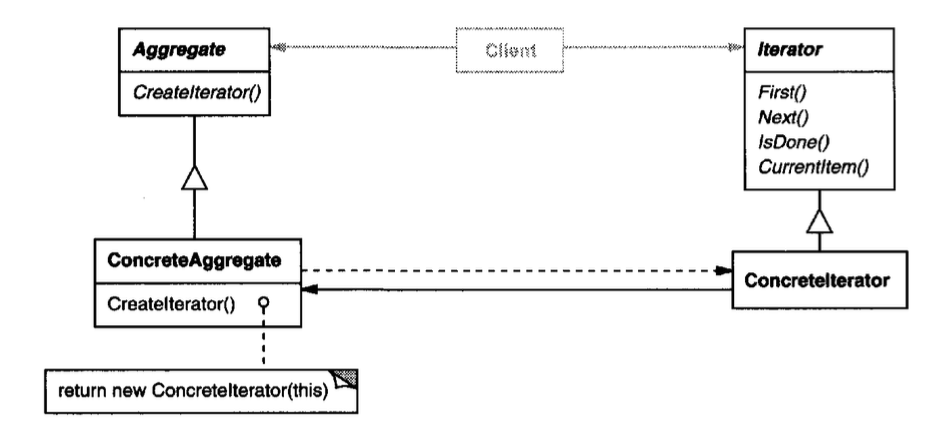
\includegraphics[width=1\linewidth]{assets/pattern/iterator/iterator-struttura.png}
    \caption{Struttura del pattern}
\end{figure}

\paragraph{Struttura} Il pattern Iterator è composto da:
\begin{itemize}
    \item \textbf{Iterator}: definisce un’interfaccia per attraversare l’insieme degli elementi di un contenitore e accedere ai singoli elementi.
    \item \textbf{ConcreteIterator}: implementa l’interfaccia Iterator tenendo traccia della posizione corrente nel contenitore e calcolando qual `e l’elemento successivo nella sequenza di attraversamento. 
    \item \textbf{Aggregate}: definisce un’interfaccia per creare un oggetto Iterator. 
    \item \textbf{ConcreteAggregate}: implementa l’interfaccia di creazione dell’Iterator e ritorna un’istanza appropriata di ConcreteIterator.
\end{itemize}

Utilizzare il pattern Iterator permette di ripulire il codice client e le collezioni di oggetti, estraendo algoritmi di attraversamento voluminosi in classi separate, ma allo stesso tempo applicare il modello può risultare eccessivo se l'applicazione utilizza solo collezioni semplici (es. Liste, Set).

\begin{figure}[H]
    \centering
    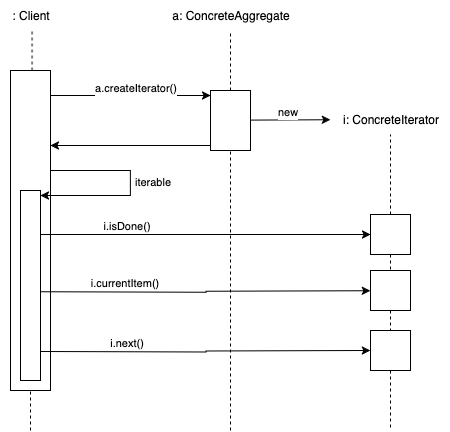
\includegraphics[width=1\linewidth]{assets/pattern/iterator/iterator-activity.drawio.png}
\end{figure}

\paragraph{Interazioni} ConcreteIterator posside un'istanza della collezione (passata a costruttore).

\newpage